\documentclass[conference]{IEEEtran}
\IEEEoverridecommandlockouts
% The preceding line is only needed to identify funding in the first footnote. If that is unneeded, please comment it out.
%Template version as of 6/27/2024

\usepackage{cite}
\usepackage{amsmath,amssymb,amsfonts}
\usepackage{algorithmic}
\usepackage{graphicx}
\usepackage{textcomp}
\usepackage{xcolor}
\usepackage{bm}
\usepackage{multirow}
\usepackage{tabularx, colortbl, makecell}
\usepackage{etoolbox}
\usepackage{hyperref}

\makeatletter
\patchcmd{\@makecaption}
  {\scshape}
  {}
  {}
  {}
\makeatother

\def\BibTeX{{\rm B\kern-.05em{\sc i\kern-.025em b}\kern-.08em
    T\kern-.1667em\lower.7ex\hbox{E}\kern-.125emX}}
\begin{document}

\title{TSELM: Target speaker extraction using discrete tokens and language models
}

\author{\IEEEauthorblockN{1\textsuperscript{st} Beilong Tang}
\IEEEauthorblockA{\textit{Duke Kunshan University} \\
% \textit{name of organization (of Aff.)}\\
Kunshan, China \\
bt132@duke.edu}
\and
\IEEEauthorblockN{2\textsuperscript{nd} Bang Zeng}
\IEEEauthorblockA{\textit{Duke Kunshan University} \\
% \textit{name of organization (of Aff.)}\\
Kunshan, China \\
zeng.bang@dukekunshan.edu.cn}
% \and
% \IEEEauthorblockN{3\textsuperscript{rd} Zhan Jin}
% \IEEEauthorblockA{\textit{Duke Kunshan University} \\
% Kunshan, China \\
% zhan.jin@whu.edu.cn}
\and
\IEEEauthorblockN{3\textsuperscript{rd} Ming Li}
\IEEEauthorblockA{\textit{Duke Kunshan University} \\
% \textit{name of organization (of Aff.)}\\
Kunshan, China \\
ming.li369@dukekunshan.edu.cn}
}

\maketitle

\begin{abstract}
  We propose TSELM, a novel target speaker extraction network that leverages discrete tokens and language models. TSELM utilizes multiple discretized layers from WavLM Large as input tokens and incorporates cross-attention mechanisms to integrate target speaker information. Language models are employed to capture the sequence dependencies, while a scalable HiFi-GAN is used to reconstruct the audio from the tokens. By applying a cross-entropy loss, TSELM models the probability distribution of output tokens, thus converting the complex regression problem of audio generation into a classification task. To the best of our knowledge, this is the first approach to target speaker extraction using discrete tokens.  The code and pretrained models are available at: \href{https://github.com/Beilong-Tang/TSELM}{https://github.com/Beilong-Tang/TSELM}.
\end{abstract}

\begin{IEEEkeywords}
target speaker extraction, speech separation, language models, audio discretization, Self-Supervised Models
\end{IEEEkeywords}
\begin{figure*}[t]
    \centering
    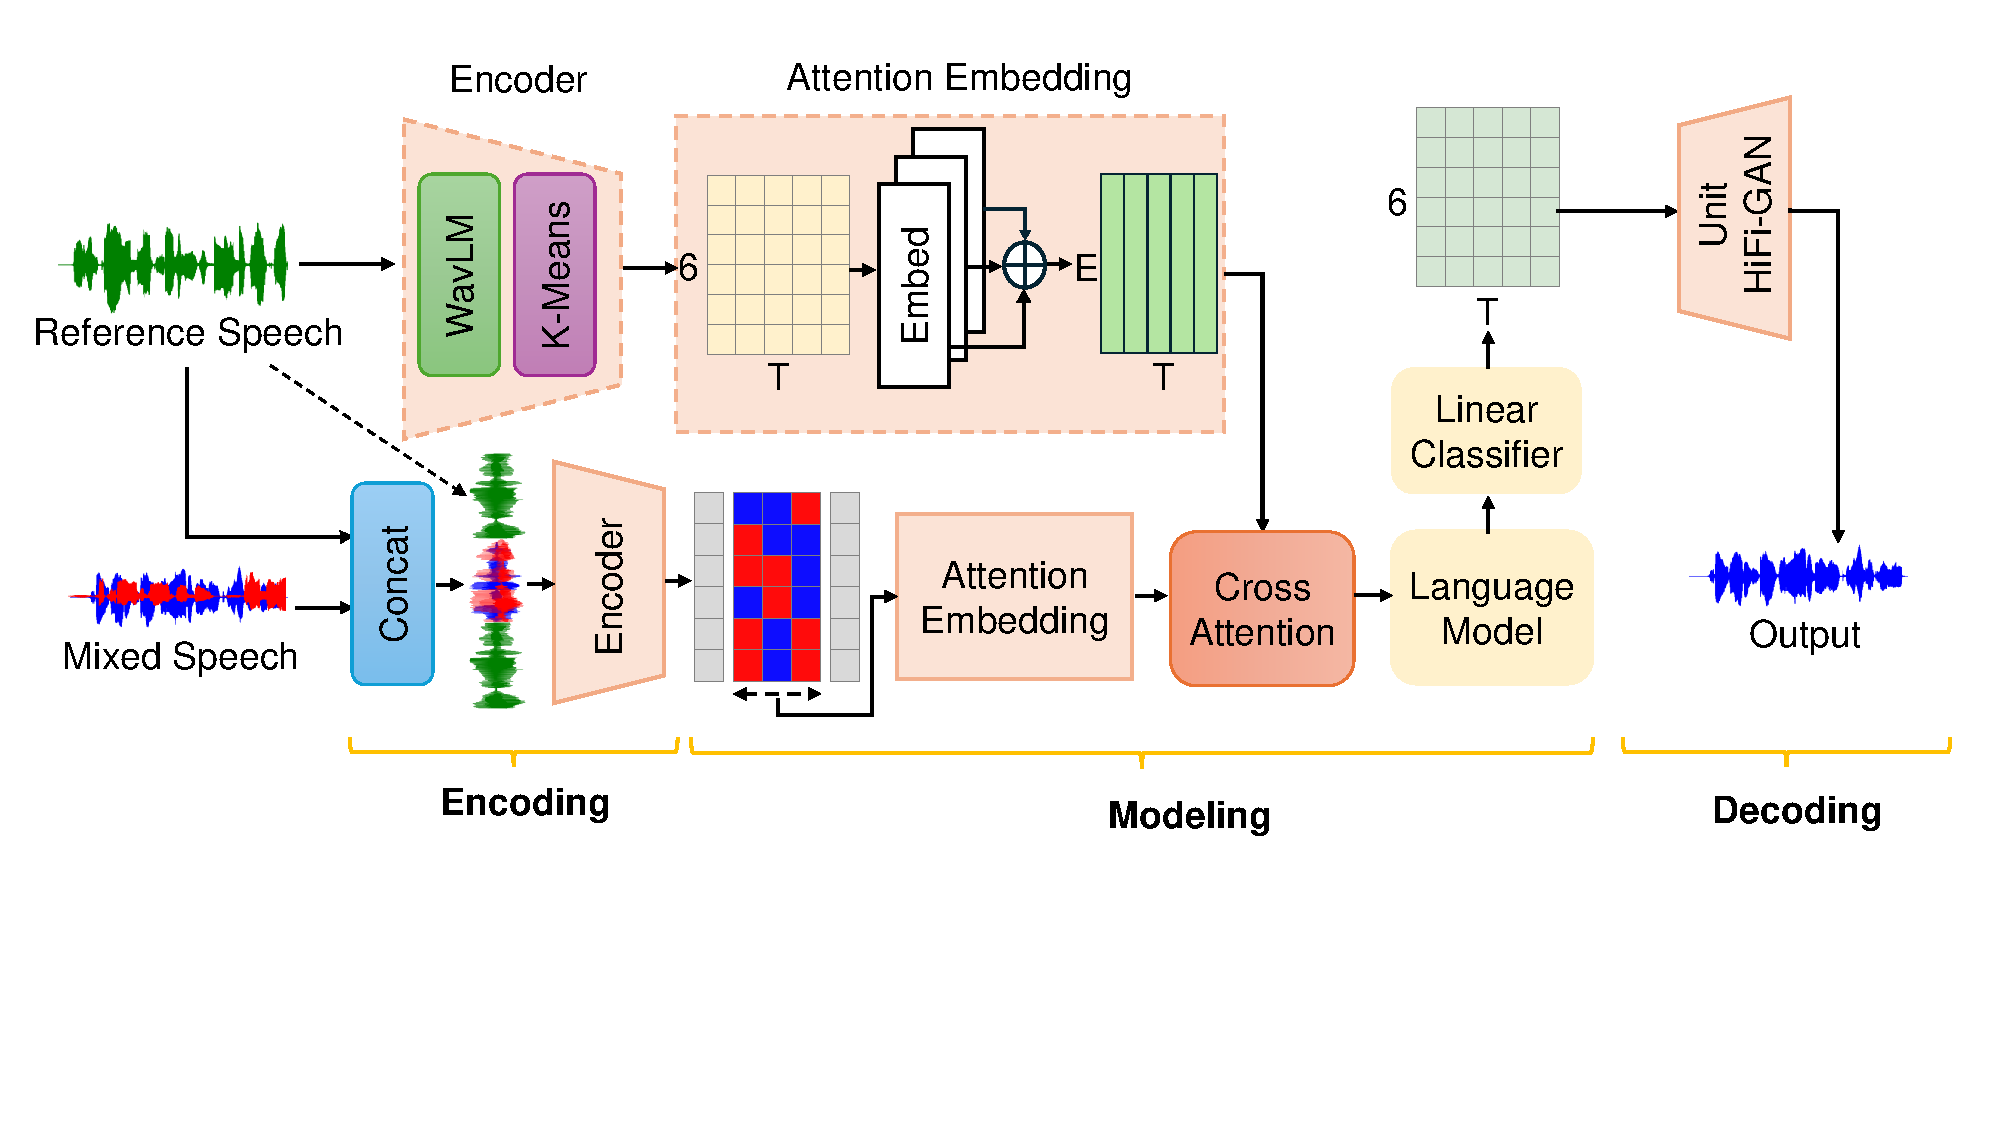
\includegraphics[width=0.77\textwidth]{assets/model.pdf}
    \caption{Overview of TSELM.}
    \label{model}
    \end{figure*}

    \begin{figure}
        \centering
        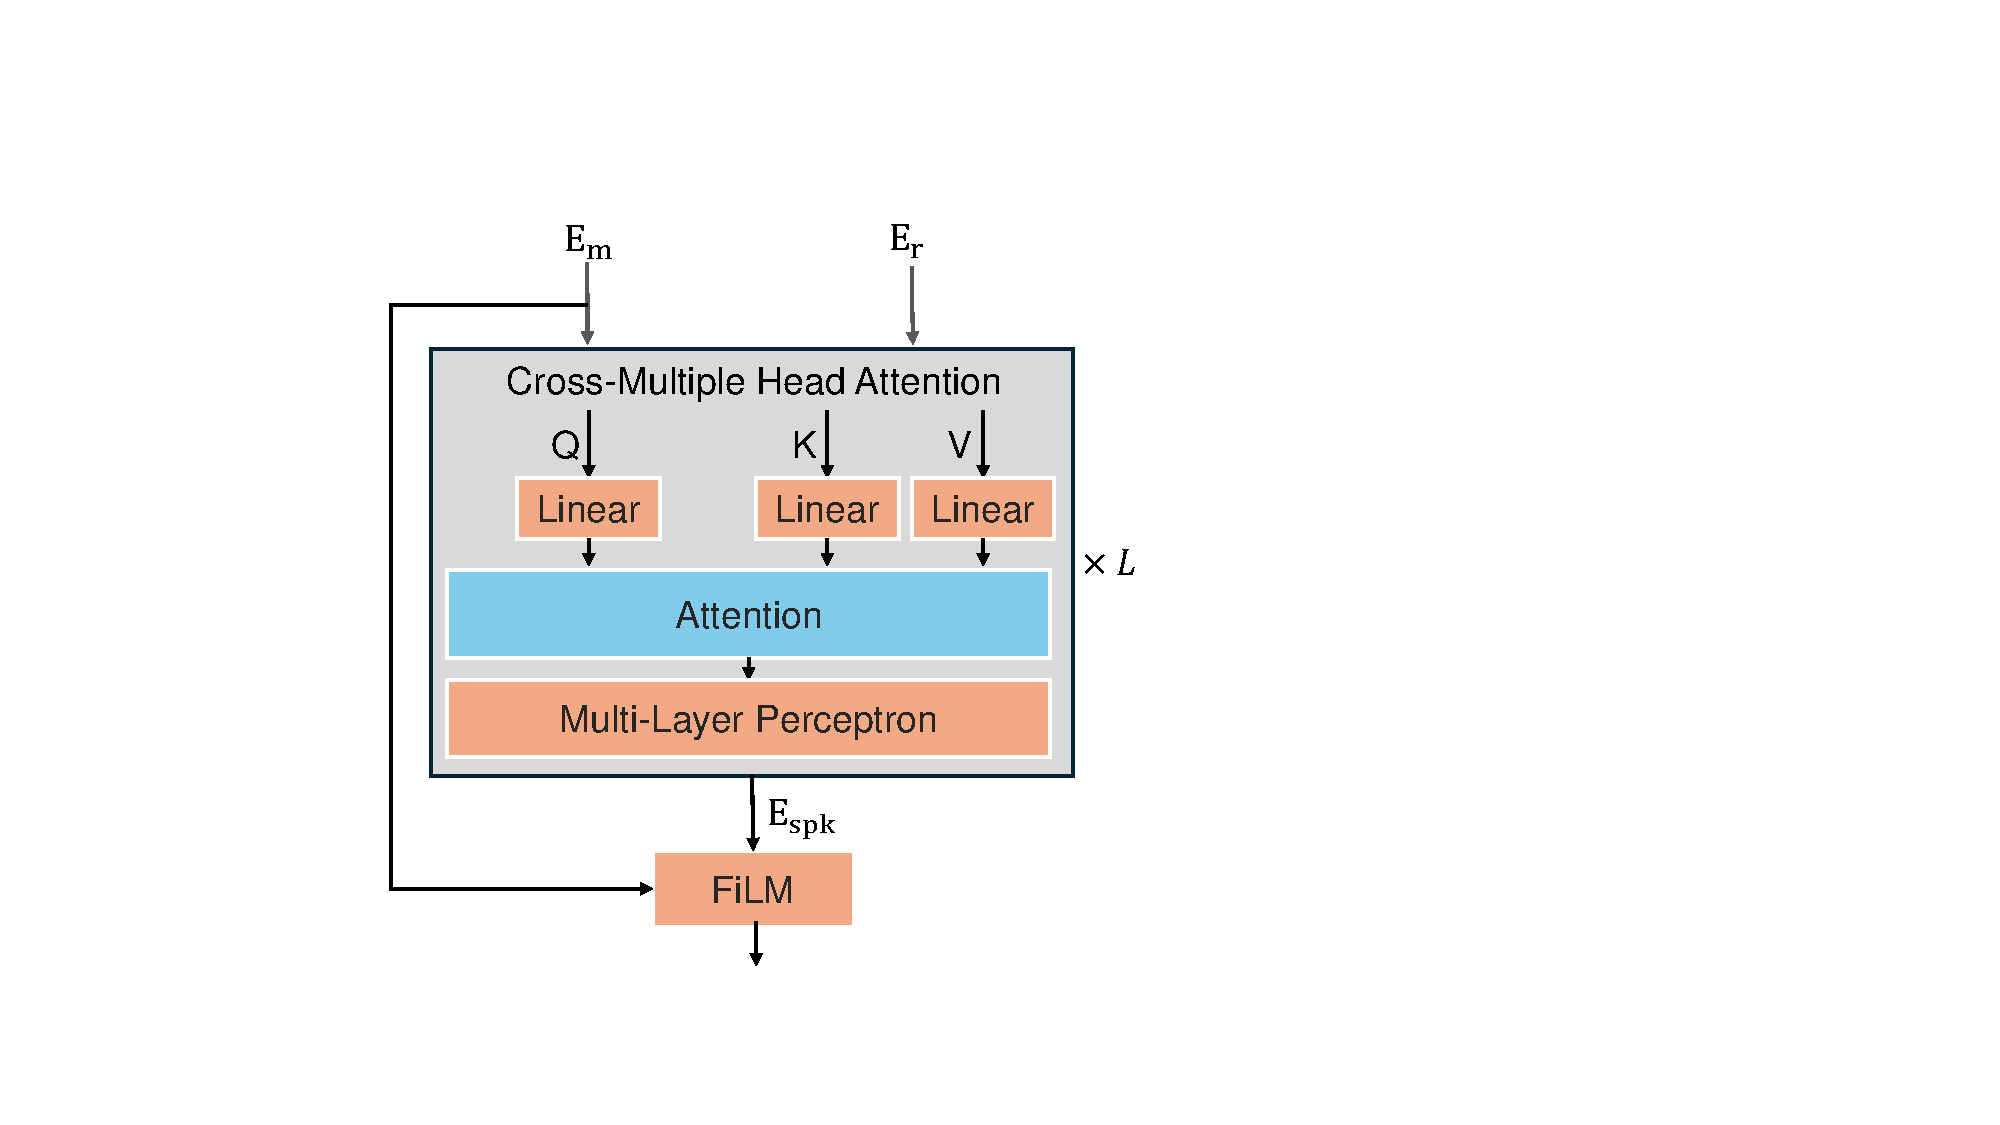
\includegraphics[width=0.25\textwidth]{assets/cross_attention.pdf}
        \caption{Details of Cross Attention mechanism.}
        \label{cross_attention}
        \end{figure}


        
\section{Introduction}

In contrast to blind speech separation, which seeks to isolate individual utterances from a mixture of known speakers, target speaker extraction (TSE) focuses on extracting only the voice of the target speaker using auxiliary information. Current models are predominantly discriminative, employing masking strategies to directly minimize the distance between the estimated and clean speech signals \cite{luo2019conv,spex_plus,sepformer,sef_net}. However, these discriminative approaches often struggle to generalize to unseen data and may introduce undesirable distortions \cite{distortion}. To address these limitations, generative models aim to learn the underlying distribution of the target speech, rather than mapping mixed speech to clean speech. Recently, generative models have been shown to achieve performance comparable to that of discriminative models in blind speech separation \cite{tokensplit} and TSE \cite{target_diff}.


The discretization of audio has gained significant attention with the advancement of language models (LMs). It has been explored in
tasks such as speech enhancement \cite{selm} and blind speech separation \cite{dasb,tokensplit}.
This method converts audio into discrete tokens, and leverages LMs to model them, thereby simplifying audio generation tasks by transforming complex regression problems into classification tasks \cite{dasb}. SSL models such as HuBERT \cite{hubert} and WavLM \cite{wavlm} have demonstrated outstanding performances across numerous downstream tasks \cite{superb}, as they extract continuous representations rich in semantic and timbral information from speech. As shown in \cite{dasb}, SSL models outperform neural audio codecs \cite{dac} in tasks like speech enhancement and separation. Consequently, this paper primarily focuses on exploring the discretization of SSL models.

The discretization approach for Target Speech Extraction (TSE) has received limited attention in the literature. One of the earliest works to introduce discrete tokens in the context of TSE is presented by \cite{gen_tse}, which investigates the use of self-supervised learning (SSL) models such as HuBERT and vq-wav2vec \cite{vq_wav2vec}. However, this study does not explore the WavLM SSL model, which has shown superior performance in speech separation tasks \cite{wavlm}. Additionally, it primarily utilizes the output from a single layer of the SSL model for discretization. Furthermore, the evaluation in \cite{gen_tse} focuses solely on speech quality, neglecting key metrics such as speech intelligibility and speaker similarity, both of which are critical for the TSE task. To address these limitations, we propose TSELM, a novel approach that leverages multiple hidden layers of WavLM for discretization and incorporates evaluation metrics for speech intelligibility and speaker similarity.

TSELM has three stages: encoding, modeling and decoding. In the encoding stage, both reference and mixed speech are tokenized using WavLM and Kmeans. The reference speech is passed directly to the encoder, while for mixed speech, we concatenate the reference speech to both sides of the mixture before passing it through the WavLM model. After tokenization, we retain only the tokens corresponding to the mixed speech.
In the modeling stage, an attention embedding mechanism is employed to combine the embeddings from all layers. A cross-attention mechanism, similar to that used in \cite{usef_tes}, is applied to inject speaker-specific information. An encoder-only language model, followed by a linear classifier, is then used to generate the reconstructed tokens.
In the decoding stage, we leverage the pretrained scalable HiFi-GAN from \cite{unit_hifi} to reconstruct the audio from the discrete tokens. Unlike SELM \cite{selm}, where a conformer detokenizer is trained to reconstruct WavLM embeddings before passing them through HiFi-GAN, the scalable HiFi-GAN in \cite{unit_hifi} uses a dropout mechanism to directly reconstruct audio from multiple layers of tokens, eliminating the need for a conformer detokenizer and the complexity of training a separate HiFi-GAN for each layer. Both the encoder and decoder are kept frozen during training, and an overview of the model is shown in Fig.\ref{model}.
Extensive experiments demonstrate that our method achieves excellent speech quality and comparable intelligibility results. To the best of our knowledge, this is the first study to explore target speaker extraction using discrete tokens. Our demos are available at \href{https://beilong-tang.github.io/TSELM.demo/}{https://beilong-tang.github.io/TSELM.demo/}.



\section{Method}
% Our model consists of three stages: encoding, modeling, and decoding. The encoder and decoder are 
% pretrained models and they are freezed during training. For the encoding stage, we use hidden layers 1, 3, 7, 12, 18, and 23 (denoted as \(n_l\)) of WavLM-Large 
% and publicly available Kmeans 
% models in \cite{dasb} to produce the discretized tokens. We use a concatenation 
% strategy to encode the mixture speech. For decoders, we use the scalable HiFi-GAN available in 
% \cite{dasb} to reconstruct the audio from discretized tokens. Our main focus is on the
% modeling stage. We apply an attention embedding mechanism to embed discrete tokens from different 
% layers into one single embedding. Encoder-only LM and linear classifier is applied afterwards to optimize the likelihood of probability 
% distribution of the clean tokens. 


\subsection{Encoding}


  % Please add the following required packages to your document preamble:
% \usepackage{multirow}


We use the pretrained self-supervised learning (SSL) model WavLM Large \cite{wavlm} to encode speech into continuous representations. Specifically, we extract the outputs from six hidden layers: 1, 3, 7, 12, 18, and 23. Given a speech signal \(s \in \mathbb{R}^{T'}\), the output of WavLM is a tensor \(\bm{r}\) with shape \(n \times T \times E\), where \(n\) is the number of output layers (6 in this case), \(T\) is the time dimension, and \(E\) represents the embedding dimension, which is 1024 in WavLM Large.  For tokenization, we apply separate Kmeans models to each output layer, with each model using the same number of clusters, denoted by \(K\). After tokenization, the continuous embedding \(\bm{r}\) is transformed into a discrete tensor \(\bm{d}\) with shape \(n \times T\), where each value \(\bm{d}_{i} \in (0, K-1) \). In all our experiments, we set \(K = 1000\). For both reference and mixed speech, the same Kmeans model and the same layer combination from WavLM Large are used. The encoder remains frozen during training.
The encoding strategy for mixed speech is crucial to the performance of the model. Given a reference speech \(s_r \in \mathbb{R}^{T^r}\) and a mixed speech \(s_m \in \mathbb{R}^{T'}\), we follow the previously described procedure to encode the reference speech into a tensor \(\bm{d_r}\) of shape \(n \times T_r\). However, for mixed speech, instead of applying the encoding directly, we first concatenate it with the reference speech, creating a signal \(s' = [s_r, s_m, s_r] \in \mathbb{R}^{(T^r + T' + T^r)}\). This concatenated signal is then input into the encoder, producing an output tensor \(\bm{d'}\) with shape \(n \times (T_r + T + T_r)\), where \(T\) represents the length for the mixed speech embedding. The tensor \(\bm{d'}\) contains discrete tokens for the two segments of reference speech and the mixed speech. We extract the portion \(\bm{d}\) corresponding to the mixed speech, resulting in an output tensor of shape \(n \times T\).

This approach is inspired by WavLM \cite{wavlm}, which trains the model by overlapping clean speech with an interfering signal covering less than 50\% of the speech, using the first utterance as the primary speaker. This allows WavLM to focus on producing target speaker dependent embeddings. Our experiments demonstrated that this concatenation strategy significantly enhances the model's performance by guiding it to prioritize the target speaker's information.
\subsection{Modeling}
\subsubsection{Attention Embedding}
After obtaining the discrete tensor \(\bm{d}\) with shape \(6 \times T\), we use 6
learnable embedding tables each with \(K\) entires to embed the 6 layers 
respectively, each resulting in a tensor of shape \(T \times E\). 
After embedding, we follow the same recipe as in \cite{dasb} to 
aggregate the tensor by using attention mechanism to sum all the 6 tensors. This summation 
keeps the information of each layer while reducing the system complexity by reducing the 
dimension of layers. After attention embedding, we obtain reference embedding \(E_r\) and 
mixture embedding \(E_m\).

\subsubsection{Cross Attention}
We apply cross attention module in \cite{usef_tes} to inject the reference embeddings into the mixture. The details 
are shown in Fig.\ref{cross_attention}.
The cross attention module consists of a stack of cross-multiple head attention modules, followed by
a feature-wise linear modulation (FiLM) module. 
We use \(E_m\) as query and \(E_r\) as key and value for 
the attention module. The output from the cross-multiple head attention module \(E_{spk}\)
is passed together with \(E_m\) to the FiLM to obtain the final output. The output of 
FiLM  \(E_f = FiLM(E_m, E_{spk}) = \gamma E_{spk} \cdot E_m  + \beta E_{spk} \) where 
\(\gamma\) and \(\beta\) are learnable parameters denoting the scaling and shifting vectors 
respectively.

\subsubsection{Language Modeling}
We use encoder-only transformers containing multiple self-attention modules to model the 
embedding \(E_f\). Due to encoder-only style, the LM is able to learn from all the positions. 
Finally, 6 linear classifiers each with dimension \(K\) is used to produce the logit scores of the tokens.
Cross-entropy loss is applied between the predicted tokens and the clean tokens, which are obtained by discretizing the ground truth clean audio.

\section{Experiments}

\subsection{Training}

We use the publicly available Kmeans tokenizer and scalable 
HiFi-GAN decoder in \cite{speechbrain}. The Kmeans tokenizer
is trained on \texttt{train\_clean\_[100,360,500]} of
LibriSpeech \cite{librispeech}, and the scalable HiFi-GAN is trained on \texttt{train\_clean\_100} of 
LibriTTS \cite{libritts}. The modeling stage is trained on 
\texttt{train\_clean\_[100,360]} of LibriSpeech. All training data are 
generated on the fly with relative SNR between 0 to 5 dB. The mixture audio and reference audio is clipped to 3 and 4 seconds, respectively.

We utilize the output from hidden layers 1, 3, 7, 12, 18, 23 from WavLM Large and Kmeans model with 
\(K=1000\).
We use embedding dimension 1024.  The cross-attention module consists of four transformer encoders, each with 16 attention heads and an MLP with a hidden dimension of 1024. Layer normalization is applied after the cross-attention module.
The LM of small version TSELM-S uses 
embedding dimension \(d\) = 256, absolute sinusoidal positional embedding, conformer encoders as backbone of LM. The conformer encoder consists of 6 layers with a kernel size of 31, each with 4 attention heads, and an MLP with a hidden dimension of 2048. The medium version TSELM-M uses \(d\) = 512 with 8 layers and 8 heads and the large version TSELM-L uses 
\(d\) = 768 with 12 layers and 16 heads. We use AdamW as 
our optimizer for all the experiments. The learning rate 
is \(5 \times 10^{-4}\) for TSELM-S and \(5 \times 10^{-5}\) for TSELM-M and TSELM-L. We train the model using 8 GPUs with 16 GB of RAM each each with batch size 16 for a total of 40,000 steps.


\subsection{Evaluation}



We use the \texttt{test} set of Libri2Mix \cite{librimix} to test our model performance and compare it with 
other baseline models. 

It is shown that metrics like PESQ, SI-SNR, STOI do not reflect speech quality of output of 
vocoders due to the fact that the vocoder output does not focus strictly on frame alignment
\cite{tokensplit,selm}. We use DNSMOS \cite{dnsmos} to measure the speech quality, and differential 
word error 
rate (dWER) \cite{dwer} to measure the speech intelligibility. For speaker similarity, we use the 
public WeSpeaker \cite{wespeaker}.


\subsection{Baseline models}
Baseline models are presented in Table \ref{main_exp}. 
TSELM is compared with Spex+ \cite{spex_plus}, a discriminative separation model trained on Libri2Mix \cite{librimix}. 
Mixture refers to the unprocessed mixed speech. 
Target-Discrete refers to the discretized target speech. It serves as the upper bond for our model.  Besides TSELM, we conduct three main experiments, named
 Continuous-WavLM-L6, TSELM-L-Hybrid and TSELM-S-NoCat using the same training data. 
For Continuous-WavLM-6, we directly
pass the embeddings from the 6th hidden layer output of WavLM Large to the cross attention  
and LM without discretization. 
The concatenation strategy is stilled applied to the mixed speech. Mean Square Error (MSE) loss is applied between the output embeddings and the clean 
embeddings. HiFi-GAN in \cite{knn_vc} is used for audio reconstruction. For 
TSELM-L-Hybrid, inspired by MaskSR \cite{mask_sr}, we discretize the reference 
speech while utilizing the continuous embeddings from the mixed speech. We call 
it hybrid because the mixture speech retains continuous features. In TSELM-S-NoCat, we utilize the TSELM-S model architecture but without concatenation strategy. 

\begin{table*}
  % \setlength{\tabcolsep}{5pt} % Adjust column spacing
  \caption{The performance of different systems on Libri2Mix testset. For TSELM-L-Hybrid  
  and TSELM, we compare the speaker similarity with the discretized target speech 
  (Target-discrete-WavLM) instead of the target speech due to the observation that 
  the process of discretization already losses the speaker information (0.653 for 
  Target-discrete-WavLM). We use "\_d" to denote it. }
  \renewcommand{\arraystretch}{1.2}
  \begin{center}
  \begin{tabular}{cccccccccccccccccc}
    \Xhline{2\arrayrulewidth} % Bold top line
  \multirow{3}{*}{System} & \multicolumn{1}{l}{\multirow{3}{*}{Category}} & \multicolumn{1}{l}{\multirow{3}{*}{Type}} &  \multicolumn{5}{c}{Libri2Mix}                    &                               & \multicolumn{5}{c}{WSJ0\_2mix}                                                  \\
  \cline{4-8} \cline{10-14}
                          & \multicolumn{1}{l}{}                                                 & \multicolumn{1}{l}{}                            & \multicolumn{3}{c}{DNSMOS $\uparrow$} & dWER $\downarrow$ & Spk Sim $\uparrow$ &  & \multicolumn{3}{c}{DNSMOS $\uparrow$} & dWER $\downarrow$ & Spk Sim $\uparrow$  \\ \cline{4-6} \cline{10-12}
                          & \multicolumn{1}{l}{}                                                    & \multicolumn{1}{l}{}                            & SIG         & BAK        & OVL        &                   &        &             & SIG         & BAK        & OVL        &                   &                    \\ \hline
  Mixture                 & -                                             & -                                                                                           & 3.39        & 3.14       & 2.68       & 79.3            & -        &           & 3.39        & 3.14       & 2.68       & 79.3            & -                  \\
  Target-Discrete         & G                                             & -                                                                                          & 3.57        & 4.10       & 3.32       & 11.3            & 0.653     &          & 3.57        & 4.10       & 3.32       & 11.3            & 0.653               \\ \hline
  Spex+                   & D                                             & -                                                                                  & 3.36        & 3.76       & 2.98       & 19.3            & 0.923     &          & 3.36        & 3.76       & 2.98       & 19.3            & 0.923             \\ \hline
  Continuous-WavLM-L6     & G                                             & C                                                                                  & 3.56        & 4.06       & 3.27       & 14.7            & 0.877     &          & 3.56        & 4.06       & 3.27       & 14.7            & 0.877             \\
  TSELM-L-Hybrid          & G                                             & H                                                                                     & 3.50        & 4.06       & 3.22       & 19.8            & 0.924\_d  &          & 3.50        & 4.06       & 3.22       & 19.8            & 0.924\_d             \\
  TSELM-S-NoCat       & G                                             & D                                                                                   & 3.47        & 4.03       & 3.19       & 69.6            & 0.868\_d    &        & 3.47        & 4.03       & 3.19       & 69.6            & 0.868\_d         \\ \hline
  TSELM-S                 & G                                             & D                                                                                    & 3.50        & 4.07       & 3.24       & 28.1            & 0.892\_d      &      & 3.50        & 4.07       & 3.24       & 28.1            & 0.892\_d            \\
  TSELM-M                 & G                                             & D                                                                                   & 3.49        & 4.05       & 3.22       & 28.4            & 0.901\_d    &        & 3.49        & 4.05       & 3.22       & 28.4            & 0.901\_d             \\
  TSELM-L                 & G                                             & D                                                                                  & 3.49        & 4.05       & 3.22       & 27.1            & 0.905\_d    &        & 3.49        & 4.05       & 3.22       & 27.1            & 0.905\_d        \\
  \Xhline{2\arrayrulewidth} % Bold top line     
  \end{tabular}
  \label{main_exp}
\end{center}
  \end{table*}

  \begin{table}
    \caption{Performance of different SSL models and layer selections. HuBERT model subsitutes the WavLM Large to HuBERT Large as the SSL model.
            The WavLM-L6 uses only the 6th layer of hidden output of WavLM Large. WavLM denotes our TSELM model which uses 6 different output layers. 
            }
            \vspace{-20.5pt}
    \renewcommand{\arraystretch}{1.1}
    \begin{center}
        \begin{tabular}{ccccccc}
            \Xhline{2\arrayrulewidth} % Bold top line
            \multirow{2}{*}{SSL-Model} & \multirow{2}{*}{Type} & \multicolumn{3}{c}{ DNSMOS $\uparrow$} & \multirow{2}{*}{dWER $\downarrow$} & \multirow{2}{*}{Spk Sim $\uparrow$} \\
            \cline{3-5}
                                                       &                             & SIG     & BAK     & OVL    &                       &                          \\ 
            \hline
            \multirow{2}{*}{HuBERT}                              &  Discrete                          & 3.56    & 4.09    & 3.30   & 81.3\%                & 0.865\_d                        \\
                                             &  Hybrid                          & 3.57    & 4.10    & 3.32   & 35.1\%                & 0.907\_d                        \\
            \hline
            \multirow{2}{*}{WavLM-L6}                              &  Discrete                          & 2.08    & 2.07    & 1.64   & 122.1\%                & 0.589\_d                        \\
            &  Hybrid                          & 3.54    & 3.84    & 3.12   & 30.0\%                & 0.849\_d                        \\
            \hline
            \multirow{2}{*}{WavLM}                                     &  Discrete                          & 3.49    & 4.05    & 3.22   & 27.1\%                & 0.905\_d                        \\
                                              &  Hybrid                          & 3.50    & 4.06    & 3.22   & 19.8\%                & 0.924\_d                        \\
            
            \Xhline{2\arrayrulewidth} % Bold top line              
            \end{tabular}
            \linebreak
            \label{hubert_wavlm_6}
      \end{center}
      \vspace{-15.5pt}
    \end{table}

\section{Results and Discussions}
Table \ref{main_exp} presents the performance of different systems evaluated on the Libri2Mix test.
The model size for Target-Discrete refers to the total size of the encoder and 
decoder, which are WavLM Large and scalable HiFi-GAN, respectively. DNSMOS is computed over the 
testset since this metric is reference-free. dWER is calculated with respect to the clean speech. 
For continuous methods, speaker similarity is directly computed against the clean speech. 
However, since discretization inherently results in some loss of speaker information—Target-Discrete shows a speaker similarity score of 0.653 compared to continuous methods—we assess the speaker similarity of the output from the discrete methods against the target audio produced by discretizing the clean speech. 
This target audio output from Target-Discrete serves as the upper bond for our model performance.
The observed speaker information loss is likely due to the tokenization process, which inherently reduces speaker fidelity. Future work should aim to enhance tokenization methods for SSL models to mitigate this loss. Since the primary goal of this research is to explore target speaker extraction using discretized information rather than to develop improved tokenization methods, we argue that comparing the outputs of our model with discretized speech is a reasonable approach, as it represents an upper bound on performance.

We observe that our model outperforms Spex+ in terms of DNSMOS scores, indicating better speech quality, but performs slightly worse in dWER, suggesting lower speech intelligibility. One potential reason for this could be the discretization process applied to the mixed speech. Our Kmeans algorithm is trained on clean speech rather than mixed speech, which is advantageous for speech enhancement as it likely aids in denoising. However, when applied to mixed speech, this discretization might lead to the model focusing on the wrong speaker, as it may only retain dominant speaker information, causing a reduction in intelligibility.
This hypothesis is supported by the results of TSELM-L-Hybrid, where continuous embeddings from the mixture speech were used without discretization, achieving dWER scores similar to Spex+. Another contributing factor could be the limitations of our current language model (LM). The encoder-only LM achieves around 50\% accuracy, and we believe using more advanced models, such as auto-regressive or masking-based LMs, could lead to improved performance in future iterations.

We observe a significant increase in dWER when the mixture audio is not concatenated with the reference, as seen in the TSELM-S-NoCat results in Table \ref{main_exp}. For WavLM to effectively perform target speaker separation, the input audio must follow specific conditions: the mixture should be less than 50\% of the total length, and the first utterance should be the target speaker. Under these conditions, WavLM outputs a slightly denoised embedding that emphasizes the target speaker. When the entire input is a mixture, however, we found that WavLM sometimes extracts the wrong speaker.
Our current concatenation strategy is inspired by SELM's \cite{selm} success in speech denoising and aims to transform the target speaker extraction task into a more difficult speech enhancement problem leveraging WavLM's denoising capability.

In Table \ref{hubert_wavlm_6}, we compare the performance of HuBERT and WavLM as SSL model and examine the effects of using either one or multiple layers for discretization. Our findings indicate that using HuBERT as the SSL model results in better DNSMOS scores but much worse dWER compared to our WavLM baseline. The improved DNSMOS scores likely stem from the vocoder performance, yet they do not adequately reflect speech intelligibility, which is crucial for speech separation tasks. 
The poorer dWER scores observed with HuBERT may be attributed to its training on clean speech, which might not equip it to capture the complexity and richness of mixed speech. Moreover, our results from WavLM-L6 suggest that when performing speech separation, discretizing across multiple layers provides better results than relying on a single layer.  This might be because that using multiple layer outputs can better tolerate errors compared to using just one layer output.

Finally, we observe a performance gap between discrete methods and continuous methods, as demonstrated by Continuous-WavLM-L6.
Continuous-WavLM-L6 has the best performance in terms of DNSMOS and dWER among all the experiments, and it only uses the 6 layer output of WavLM. 
It has a better dWER of 13.6\% compared with TSELM-L. The gap in performance may be attributed to the information loss inherent in the discretization process. 
We hope future research will work to bridge this gap.   

\section{Conclusion}
In this work, we introduced a novel way using discrete tokens and language models for target speaker extraction.
Our method leverages multiple hidden layers of WavLM and Kmeans tokenizers for encoding, employs cross-attention and a language model for separation, and utilizes a scalable HiFi-GAN for audio reconstruction.
Experiments have 
shown that our model can achieve excellent performance in terms of speech quality, and comparable performance in terms of speech intelligibility and 
speaker similarity. However, we still have a gap between continuous methods especially in speech intelligibility and speaker similarity. Future research should focus on shrinking 
this gap. 

\section{Acknowledgment}
We want to thank Super Computing Network (SCNet) for providing the computing resources. 


% \section*{Acknowledgment}

% We want to thank for Kunshan Super Computing SCNet for providing the computing resources. 

\bibliographystyle{IEEEtran}
\bibliography{references}


\end{document}
